\chapter{Paired Three-Dimensional Particle--Mesh Nonlinear Refinement}
\label{ch:paired-pm-nonlinear}

\section{Scope and objective}

The preceding nonlinear-structure chapter propagated the collisionless refinement transfer through spherical collapse, a halo mass function, a compensated halo model, and reionization consistency.  That calculation found that nonlinear halo formation can regenerate much of the linearly suppressed small-scale power, while low-mass halo abundance and formation time remain more strongly altered.  The result was model based rather than a direct phase-space evolution.

This chapter supplies an independent test.  It evolves paired cold and refinement initial conditions with the same random phases in a three-dimensional cosmological particle--mesh system.  The calculation is designed to answer three narrow questions:
\begin{enumerate}[leftmargin=2em]
\item Does direct nonlinear evolution regenerate the suppressed refinement power?
\item Does delayed high-density collapse remain visible after that regeneration?
\item Does an independent particle calculation agree with the preceding halo-model trend?
\end{enumerate}

The answer to all three questions is affirmative in the declared finite box.  The calculation is a controlled particle--mesh benchmark.  It is not a precision $N$-body simulation, a resolved subhalo catalog, or an observational likelihood.

\section{Paired initial conditions}

Let $P_{\rm c}(k)$ denote the cold linear power normalized to $\sigma_8=0.81$.  The refinement branch uses the previously derived collisionless transfer amplitude $T_D(k)$,
\begin{equation}
 P_D(k)=T_D(k)^2P_{\rm c}(k),
 \qquad 0\leq T_D(k)\leq1.
 \label{eq:pm-paired-linear-power}
\end{equation}
The same Gaussian white-noise realization is used in both branches.  Thus every retained Fourier mode has the same initial phase.  Before nonlinear evolution,
\begin{equation}
 r_{\rm cD}(k)
 :=
 \frac{P_{\rm cD}(k)}{\sqrt{P_{\rm c}(k)P_D(k)}}=1,
 \label{eq:pm-initial-cross-correlation}
\end{equation}
and the only difference is the deterministic amplitude factor $T_D(k)$.

The Zel'dovich map is
\begin{equation}
 \boldsymbol x(\boldsymbol q,a_i)
 =
 \boldsymbol q+D(a_i)\boldsymbol s(\boldsymbol q),
 \label{eq:pm-zeldovich-position}
\end{equation}
\begin{equation}
 \boldsymbol p(\boldsymbol q,a_i)
 =
 a_i^2H(a_i)f(a_i)D(a_i)\boldsymbol s(\boldsymbol q),
 \label{eq:pm-zeldovich-momentum}
\end{equation}
where
\begin{equation}
 \boldsymbol s_{\boldsymbol k}
 =
 i\frac{\boldsymbol k}{k^2}\delta_{0,\boldsymbol k},
 \qquad
 f=\frac{d\log D}{d\log a}.
 \label{eq:pm-zeldovich-displacement}
\end{equation}
The background uses
\begin{equation}
 E(a)^2
 =
 \Omega_{r0}a^{-4}
 +\Omega_{m0}a^{-3}
 +\Omega_{V0},
 \label{eq:pm-background}
\end{equation}
with
\begin{equation}
 \Omega_{m0}=0.31,
 \qquad
 \Omega_{r0}=9\times10^{-5},
 \qquad
 \Omega_{V0}=0.68991.
 \label{eq:pm-background-values}
\end{equation}

\section{Particle--mesh evolution}

In comoving coordinates,
\begin{equation}
 \ddot{\boldsymbol x}+2H\dot{\boldsymbol x}
 =
 -\frac{1}{a^2}\nabla_x\Phi,
 \label{eq:pm-comoving-equation}
\end{equation}
\begin{equation}
 \nabla_x^2\Phi
 =
 \frac32\Omega_{m0}H_0^2a^{-1}\delta.
 \label{eq:pm-poisson}
\end{equation}
Define the canonical momentum
\begin{equation}
 \boldsymbol p=a^2\dot{\boldsymbol x}.
 \label{eq:pm-canonical-momentum}
\end{equation}
Using the scale factor as time gives
\begin{equation}
 \frac{d\boldsymbol x}{da}
 =
 \frac{\boldsymbol p}{a^3H},
 \label{eq:pm-drift-equation}
\end{equation}
\begin{equation}
 \frac{d\boldsymbol p}{da}
 =
 \frac{3\Omega_{m0}H_0^2}{2a^2H}
 \nabla\nabla^{-2}\delta.
 \label{eq:pm-kick-equation}
\end{equation}

Cloud-in-cell deposition defines the mesh density.  The Fourier-space mesh force is
\begin{equation}
 \boldsymbol F_{\boldsymbol k}
 =
 i\frac{\boldsymbol k}{k^2}\delta_{\boldsymbol k},
 \qquad \boldsymbol F_{\boldsymbol 0}=0.
 \label{eq:pm-spectral-force}
\end{equation}
The same cloud-in-cell kernel interpolates the force back to the particles.  This symmetric assignment keeps the net force and total canonical momentum at roundoff.

The kick--drift--kick factors are evaluated by Gaussian quadrature,
\begin{equation}
 K(a_1,a_2)
 =
 \frac32\Omega_{m0}
 \int_{a_1}^{a_2}
 \frac{da}{a^2E(a)},
 \label{eq:pm-kick-factor}
\end{equation}
\begin{equation}
 D_{\rm drift}(a_1,a_2)
 =
 \int_{a_1}^{a_2}
 \frac{da}{a^3E(a)}.
 \label{eq:pm-drift-factor}
\end{equation}

\section{Numerical realization}

The main paired calculation uses
\begin{equation}
 N_g=64,
 \qquad
 N_p=64^3=262144,
 \label{eq:pm-main-resolution}
\end{equation}
\begin{equation}
 L=14.2857142857\ {\rm Mpc},
 \qquad
 \Delta x=0.2232142857\ {\rm Mpc},
 \label{eq:pm-box}
\end{equation}
\begin{equation}
 a_i=0.02,
 \qquad
 N_{\rm step}=80.
 \label{eq:pm-time-resolution}
\end{equation}
The particle mass is
\begin{equation}
 m_p
 =
 \bar\rho_m\frac{L^3}{N_p}
 =
 4.6886092251\times10^8\ M_\odot.
 \label{eq:pm-particle-mass}
\end{equation}
The deconvolved power analysis retains
\begin{equation}
 k<0.65k_{\rm Ny}
 =9.1483178073\ {\rm Mpc}^{-1}.
 \label{eq:pm-usable-k}
\end{equation}
The input power half-mode is
\begin{equation}
 k_{1/2}=7.3571107668\ {\rm Mpc}^{-1},
 \label{eq:pm-input-half-mode}
\end{equation}
so the main mesh resolves the declared cutoff region.

\section{Nonlinear power regeneration}

For each snapshot define
\begin{equation}
 R_P(k,a)
 :=
 \frac{P_D^{\rm PM}(k,a)}{P_{\rm c}^{\rm PM}(k,a)}.
 \label{eq:pm-power-ratio}
\end{equation}
At $k=8\ {\rm Mpc}^{-1}$, the input linear ratio is
\begin{equation}
 T_D(8)^2=0.4474940507.
 \label{eq:pm-k8-input}
\end{equation}
The measured paired ratios are
\begin{align}
 R_P(8,0.05)&=0.5236906387,\label{eq:pm-k8-a005}\\
 R_P(8,0.10)&=0.6336086860,\label{eq:pm-k8-a01}\\
 R_P(8,0.25)&=0.9082585376,\label{eq:pm-k8-a025}\\
 R_P(8,0.50)&=0.9567667002,\label{eq:pm-k8-a05}\\
 R_P(8,1)&=0.9918100525.\label{eq:pm-k8-a1}
\end{align}
At the input half-mode,
\begin{equation}
 R_P(k_{1/2},1)=0.9928833783.
 \label{eq:pm-halfmode-final}
\end{equation}
The direct particle evolution therefore confirms the earlier conclusion:
\begin{equation}
 \boxed{
 \text{nonlinear mode coupling regenerates most of the linearly suppressed power by }a=1.
 }
 \label{eq:pm-regeneration-conclusion}
\end{equation}

\begin{figure}[htbp]
\centering
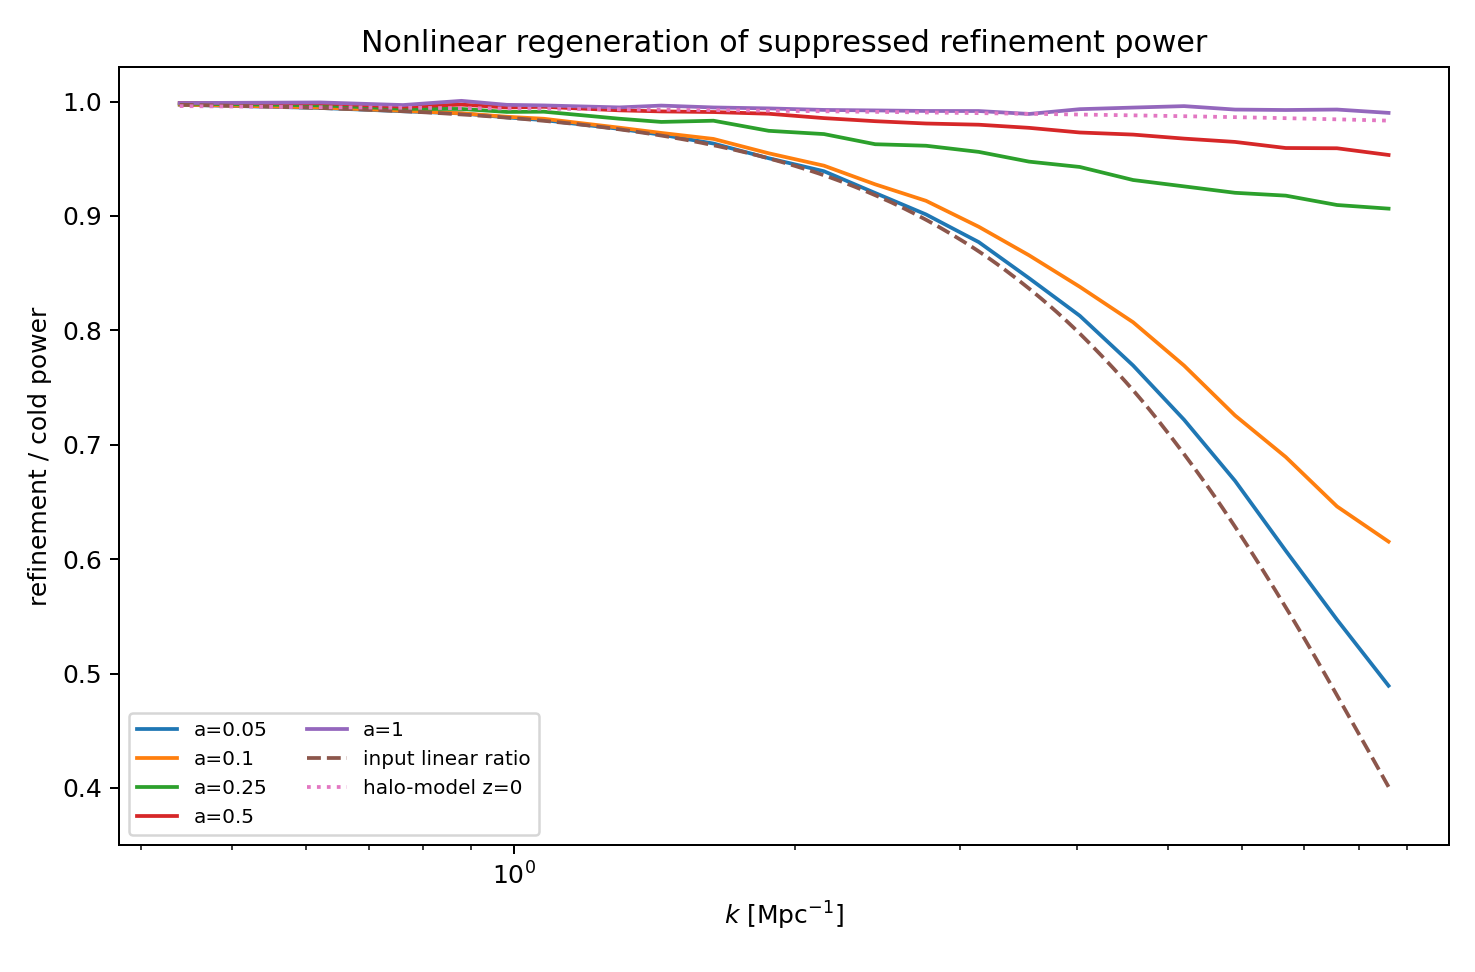
\includegraphics[width=0.95\linewidth]{figures/pm/01_power_regeneration.png}
\caption{Paired nonlinear power ratios.  The early evolution retains the linear cutoff.  The ratio approaches unity as nonlinear mode coupling transfers power into the suppressed band.  The independent halo-model result has the same late-time trend.}
\label{fig:pm-power-regeneration}
\end{figure}

Selected values are collected below.
\begin{center}
\begin{tabular}{rrrrr}
\toprule
$k\,[{\rm Mpc}^{-1}]$ & input $T_D^2$ & $R_P(a=0.05)$ & $R_P(a=0.25)$ & $R_P(a=1)$\\
\midrule
4.00 & 0.79954 & 0.81467 & 0.94307 & 0.99307\\
6.00 & 0.61937 & 0.66078 & 0.91991 & 0.99292\\
7.35 & 0.50060 & 0.56281 & 0.91169 & 0.99288\\
8.00 & 0.44749 & 0.52369 & 0.90826 & 0.99181\\
9.00 & 0.37277 & 0.48933 & 0.90637 & 0.99008\\
\bottomrule
\end{tabular}
\end{center}

\section{Phase coherence of the nonlinear cosmic web}

The paired cross-correlation is
\begin{equation}
 r_{\rm cD}(k,a)
 =
 \frac{P_{\rm cD}(k,a)}{
 \sqrt{P_{\rm c}(k,a)P_D(k,a)}}.
 \label{eq:pm-cross-correlation}
\end{equation}
At $k=8\ {\rm Mpc}^{-1}$,
\begin{equation}
 r_{\rm cD}(8,1)=0.9981981720.
 \label{eq:pm-k8-cross}
\end{equation}
Across the retained $a=1$ modes,
\begin{equation}
 \min_k r_{\rm cD}(k,1)=0.9978380.
 \label{eq:pm-min-cross}
\end{equation}
The large-scale skeleton and most nonlinear structures therefore remain paired.  The refinement branch alters collapse timing and internal density more strongly than it relocates the cosmic web.

\begin{figure}[htbp]
\centering
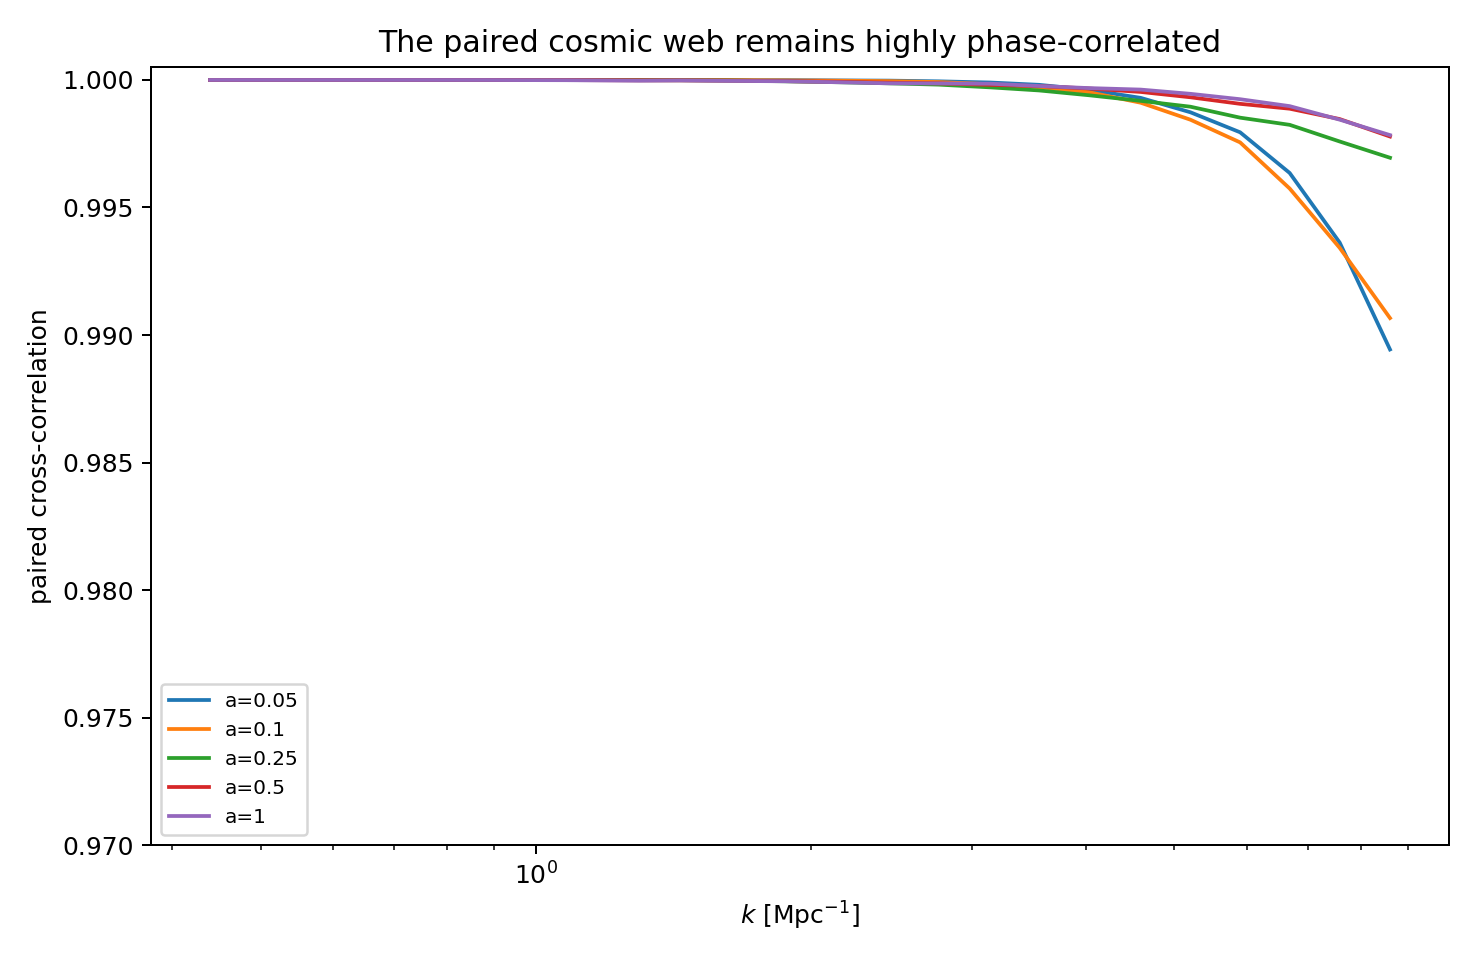
\includegraphics[width=0.95\linewidth]{figures/pm/03_cross_correlation.png}
\caption{Cross-correlation of the paired density fields.  The phases remain highly correlated even after nonlinear power has been regenerated.}
\label{fig:pm-cross-correlation}
\end{figure}

\begin{figure}[htbp]
\centering
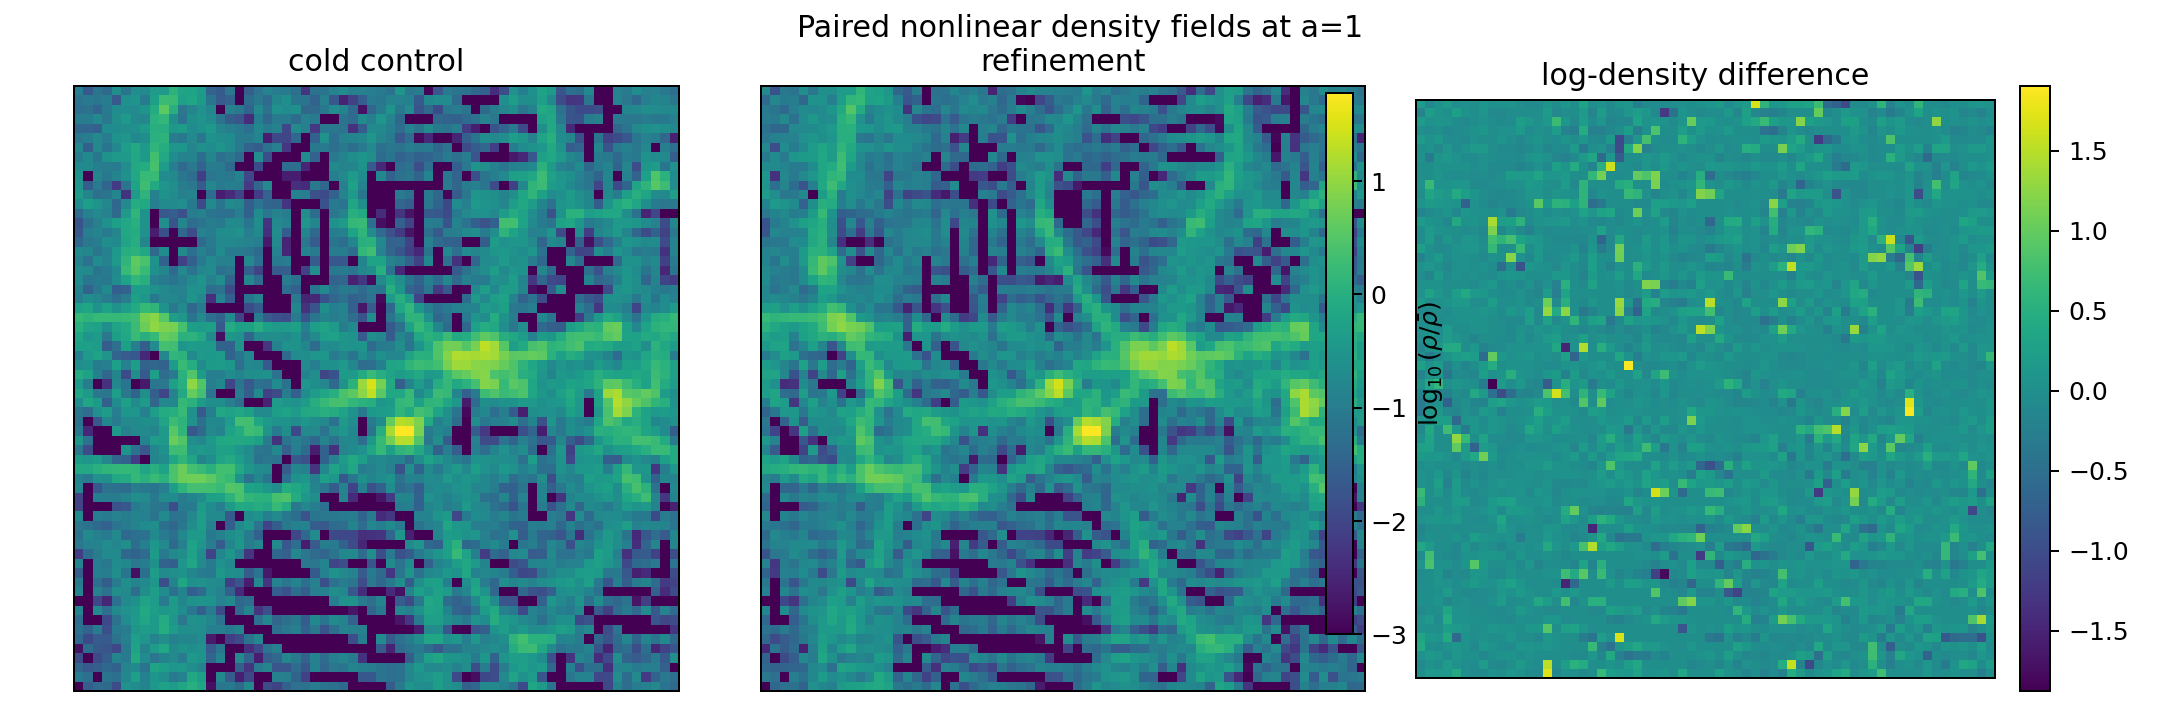
\includegraphics[width=\linewidth]{figures/pm/04_density_slices.png}
\caption{Four-cell slab averages of the paired $a=1$ density fields.  The same filaments and nodes appear in both branches, while the difference map isolates changes in local collapse and internal density.}
\label{fig:pm-density-slices}
\end{figure}

\section{Delayed high-density collapse}

For a mesh density threshold $\Delta_\rho$, define the mass fraction
\begin{equation}
 F_M(>\Delta_\rho,a)
 =
 \frac{
 \sum_{j:\rho_j/\bar\rho>\Delta_\rho}\rho_j
 }{
 \sum_j\rho_j
 }.
 \label{eq:pm-collapsed-mass-fraction}
\end{equation}
A local mesh maximum above the same threshold is counted as a peak proxy.  These are not halo catalogs.  They provide a direct, resolution-declared collapse diagnostic.

At $a=0.25$, corresponding to $z=3$, the threshold $\rho/\bar\rho>20$ gives
\begin{equation}
 \frac{F_{M,D}}{F_{M,\rm c}}=0.9045351965,
 \label{eq:pm-z3-mass-ratio}
\end{equation}
\begin{equation}
 \frac{N_{{\rm peak},D}}{N_{{\rm peak},\rm c}}=0.8551724138.
 \label{eq:pm-z3-peak-ratio}
\end{equation}
At $a=1$, the corresponding ratios are
\begin{equation}
 \frac{F_{M,D}}{F_{M,\rm c}}=0.9745091917,
 \qquad
 \frac{N_{{\rm peak},D}}{N_{{\rm peak},\rm c}}=0.8962962963.
 \label{eq:pm-z0-collapse-ratios}
\end{equation}
Power regeneration is therefore more complete than collapse-statistic regeneration.

\begin{figure}[htbp]
\centering
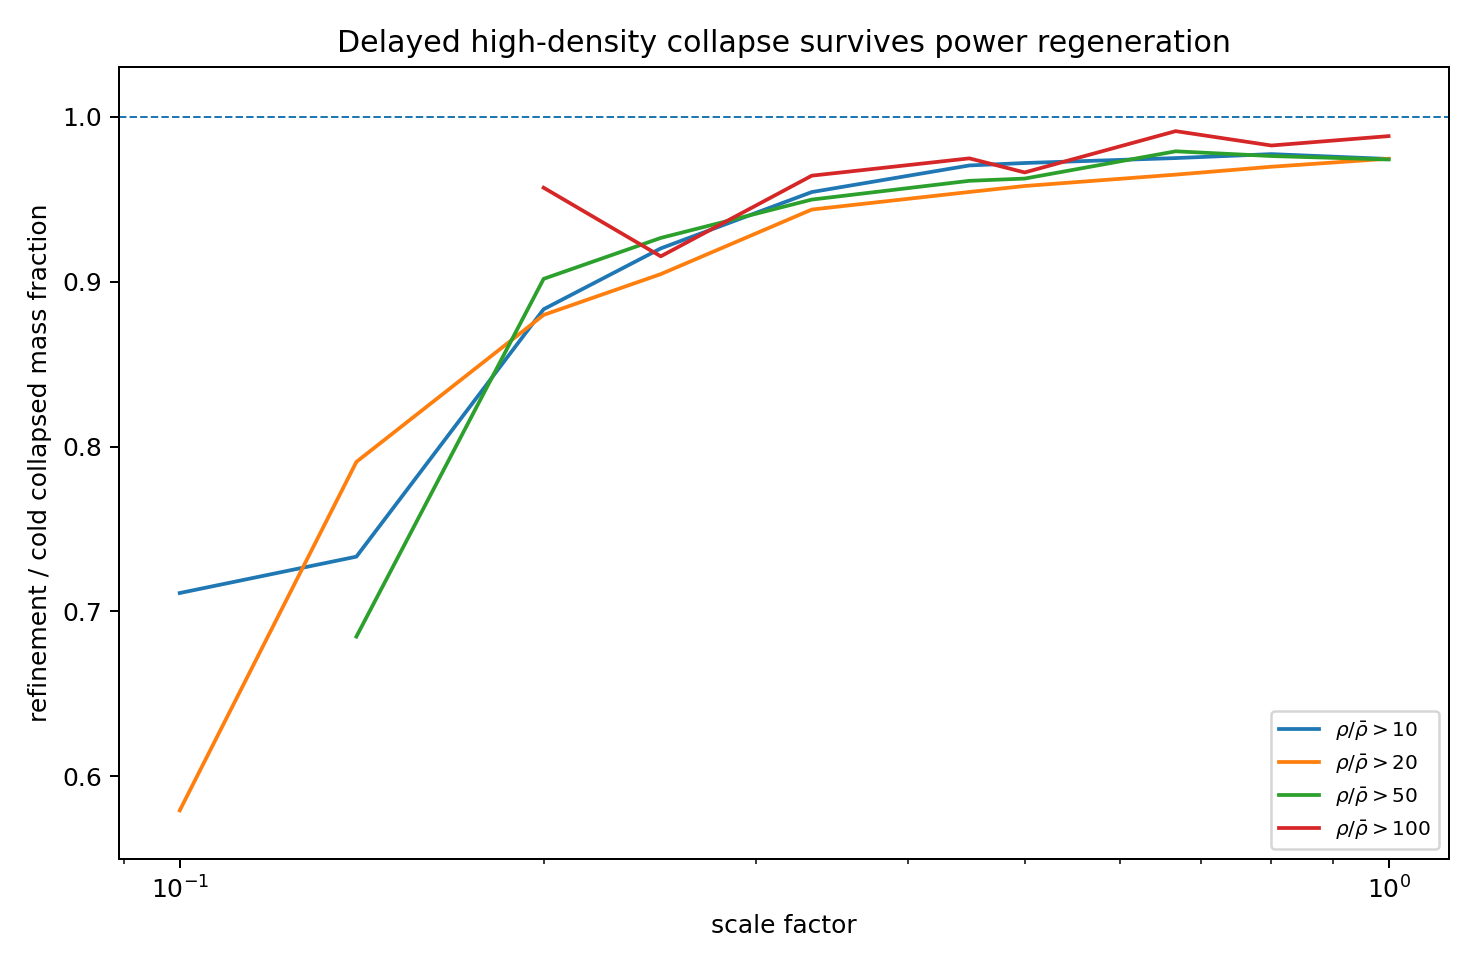
\includegraphics[width=0.95\linewidth]{figures/pm/02_collapsed_mass_fraction.png}
\caption{Ratio of refinement to cold mass above fixed mesh-density thresholds.  The largest delay occurs during the onset of nonlinear collapse.  The ratios approach unity at late times but do not become exactly equal.}
\label{fig:pm-collapsed-fraction}
\end{figure}

For selected target mass fractions, the interpolation gives:
\begin{center}
\begin{tabular}{rrrrr}
\toprule
threshold & target $F_M$ & $a_{\rm c}$ & $a_D$ & delay $a_D/a_{\rm c}-1$\\
\midrule
10 & 0.25 & 0.29540 & 0.30615 & 0.03641\\
20 & 0.10 & 0.24093 & 0.25122 & 0.04270\\
50 & 0.10 & 0.33546 & 0.34352 & 0.02405\\
100 & 0.05 & 0.32301 & 0.32749 & 0.01386\\
\bottomrule
\end{tabular}
\end{center}
Thus the controlled formation delay is of order one to four percent in scale factor for these mesh thresholds.

\section{Independent comparison with the halo-model closure}

The preceding compensated halo model predicted a mild $z=0$ nonlinear suppression despite a strong linear cutoff.  The particle--mesh and halo-model ratios are independent constructions.  Their root-mean-square difference over the common retained modes is
\begin{equation}
 \boxed{
 \epsilon_{\rm PM/HM}=4.6838158064\times10^{-3}.
 }
 \label{eq:pm-halo-rms}
\end{equation}
At $k=8\ {\rm Mpc}^{-1}$,
\begin{equation}
 R_P^{\rm PM}=0.9918100525,
 \qquad
 R_P^{\rm halo}=0.9839760245.
 \label{eq:pm-halo-k8}
\end{equation}
The agreement is not a proof that either approximation is precision accurate.  It is a nontrivial cross-method confirmation of the same qualitative conclusion:
\begin{equation}
 \boxed{
 \begin{gathered}
 \text{late-time power can nearly recover,}\\
 \text{while halo and peak statistics retain a stronger memory of the cutoff.}
 \end{gathered}
 }
 \label{eq:pm-cross-method-conclusion}
\end{equation}

\section{Verification and convergence}

The deterministic audit records
\begin{equation}
 \boxed{20\ {\rm PASS},\qquad0\ {\rm FAIL}.}
 \label{eq:pm-audit-total}
\end{equation}
Selected controls are:
\begin{center}
\begin{tabular}{lr}
\toprule
control & residual or discrepancy\\
\midrule
mass conservation & $4.16\times10^{-17}$\\
maximum mean net force & $4.31\times10^{-15}$\\
relative total-momentum residual & $7.21\times10^{-16}$\\
linear plane-wave growth error & $7.49\times10^{-3}$\\
grid-control ratio discrepancy & $1.67\times10^{-2}$\\
time-step ratio discrepancy & $1.11\times10^{-3}$\\
paired-phase fractional scatter & $2.79\times10^{-3}$\\
PM versus halo-model RMS difference & $4.68\times10^{-3}$\\
\bottomrule
\end{tabular}
\end{center}
The $48^3$ grid control and the 96-step time control preserve the paired ratios within the declared tolerances.  Two independent paired-phase runs on a smaller grid give sub-percent ratio scatter.

\section{Physical interpretation}

The direct particle calculation changes the emphasis of the refinement prediction.

First, a large suppression in the linear transfer does not imply an equally large suppression in the fully nonlinear matter power.  Mode coupling and collapse repopulate the high-$k$ band.

Second, the initial cutoff still has measurable dynamical consequences.  High-density regions appear later, contain slightly less mass, and contain fewer mesh peaks.  These effects are strongest during early nonlinear formation and persist weakly to the present.

Third, the paired fields remain almost perfectly phase correlated.  The candidate model predicts a familiar large-scale cosmic web with altered low-mass and internal structure, rather than a radically relocated web.

The strongest controlled conclusion is therefore
\begin{equation}
 \boxed{
 \begin{gathered}
 \text{linear cutoff}\
 \Downarrow\\
 \text{delayed early collapse and fewer dense peaks}\
 \Downarrow\\
 \text{nonlinear high-}k\text{ power regeneration}\
 \Downarrow\\
 \text{late-time power nearly cold, but formation memory remains}.
 \end{gathered}
 }
 \label{eq:pm-physical-chain}
\end{equation}

\section{Claim boundary}

The calculation has several explicit limitations.
\begin{itemize}[leftmargin=2em]
\item The box is $14.29\ {\rm Mpc}$ on a side and omits long-wavelength sample variance.
\item The force is particle--mesh with a $0.223\ {\rm Mpc}$ cell.  Halo cores and subhalos are unresolved.
\item The particle mass is $4.69\times10^8M_\odot$.  The run cannot directly test the smallest halo masses in the analytic mass-function calculation.
\item The initial conditions use the Zel'dovich approximation rather than a production-grade second-order generator.
\item There is no baryonic gas, cooling, star formation, feedback, or radiation transport.
\item The mesh peak statistic is not a friends-of-friends or spherical-overdensity halo finder.
\item One finite box does not establish a converged cosmological prediction.
\end{itemize}

The result is therefore a controlled nonlinear phase-space benchmark, not a final simulation campaign.
